% Classes of src/core/Math/Derivative and their dependencies. Paper: section "Interpolation, integration and
% differentiation" (fig:derivative); Doxygen: Differentiation.hpp.
%   pdflatex DerivativeClasses.tex; pdftoppm -r 200 -png -singlefile DerivativeClasses.pdf DerivativeClasses;
%   pdftocairo -svg DerivativeClasses.pdf DerivativeClasses.svg
\documentclass[tikz,border=2pt]{standalone}
% Shared style of the class diagrams of CAP (figures/*Classes.tex): \input after \documentclass[tikz]{standalone}.
%  - boxes: blue = abstract base class, light blue = class, green = entry class of the folder (steering class, task),
%    yellow = free functions (tools), grey = class of another folder;
%  - arrows: open triangle = inherits from; dashed with diamond = owns (holds); dashed with arrow = uses.
\usepackage[scaled=0.92]{helvet}
\usetikzlibrary{arrows.meta,shapes.multipart,positioning,fit,backgrounds,calc}
\renewcommand{\familydefault}{\sfdefault}
\definecolor{abstract}{HTML}{D6E4F5}
\definecolor{concrete}{HTML}{EEF4FB}
\definecolor{steer}{HTML}{DCEFD9}
\definecolor{tools}{HTML}{FFF8E6}
\definecolor{external}{HTML}{E9E9E9}
\definecolor{dependline}{HTML}{8A6D3B}
\definecolor{folder}{HTML}{F7F7F7}
\tikzset{
  every picture/.style={font=\scriptsize},
  cls/.style={draw, fill=concrete, align=center, inner sep=2.5pt, text width=#1, font=\tiny},
  cls/.default=3.0cm,
  abs/.style={cls=#1, fill=abstract},
  abs/.default=3.0cm,
  steer/.style={cls=#1, fill=steer, line width=0.8pt},
  steer/.default=4.2cm,
  tool/.style={cls=#1, fill=tools},
  tool/.default=4.2cm,
  ext/.style={cls=#1, fill=external, dashed},
  ext/.default=2.6cm,
  fam/.style={draw, rectangle split, rectangle split parts=2, rectangle split part fill={#1,white},
              rectangle split part align={center,left}, inner sep=2.5pt, align=left},
  inherit/.style={-{Triangle[open,length=2.2mm,width=2.2mm]}, thin},
  uses/.style={dashed, dependline, -{Stealth[length=1.6mm]}, thin},
  owns/.style={dashed, dependline, {Diamond[length=2.4mm,width=1.6mm]}-, thin},
  lbl/.style={font=\tiny, text=dependline, align=center},
  note/.style={font=\tiny, align=left, text=black!70},
  title/.style={font=\footnotesize\bfseries, anchor=north west},
}
% a member line in a class box
\newcommand{\m}[1]{\\#1}
\newcommand{\cn}[1]{{\scriptsize\textbf{#1}}}
\newcommand{\an}[1]{{\scriptsize\textbf{\textit{#1}}}}

% legend common to the class diagrams (place with \legendat{x}{y})
\newcommand{\legendat}[2]{%
  \begin{scope}[shift={(#1,#2)}, font=\tiny]
    \node[abs=0.9cm, minimum height=3mm, inner sep=1pt] (lA) at (0,0) {abstract};
    \node[cls=0.9cm, minimum height=3mm, inner sep=1pt, right=1mm of lA] (lC) {class};
    \node[steer=1.1cm, minimum height=3mm, inner sep=1pt, right=1mm of lC] (lS) {entry class};
    \node[tool=1.1cm, minimum height=3mm, inner sep=1pt, right=1mm of lS] (lT) {functions};
    \node[ext=1.3cm, minimum height=3mm, inner sep=1pt, right=1mm of lT] (lE) {other folder};
    \draw[inherit] ($(lE.east)+(1mm,0)$) -- ++(5mm,0) node[right, inner sep=1pt] (l1) {inherits};
    \draw[owns] ($(l1.east)+(1mm,0)$) -- ++(5mm,0) node[right, inner sep=1pt] (l2) {owns};
    \draw[uses] ($(l2.east)+(1mm,0)$) -- ++(5mm,0) node[right, inner sep=1pt] {uses};
  \end{scope}}

\begin{document}
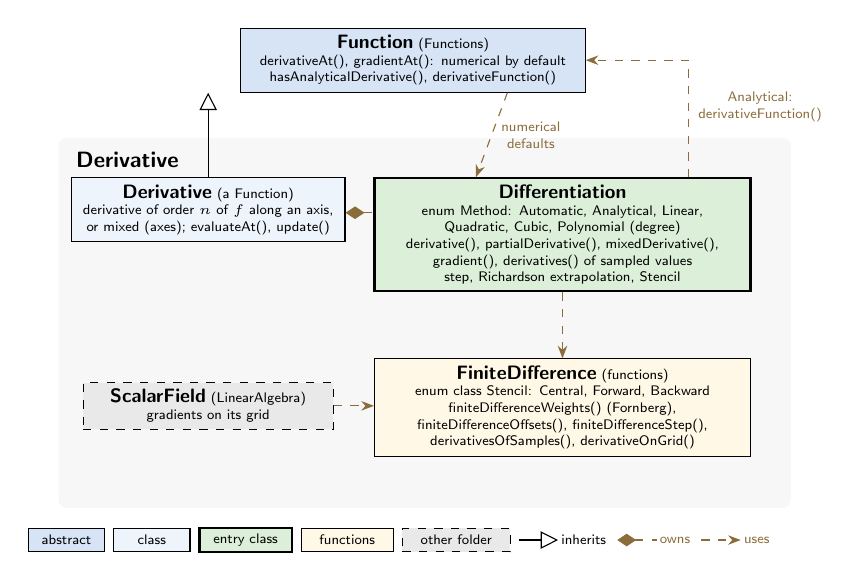
\begin{tikzpicture}[every node/.append style={anchor=north}]
  \begin{scope}[on background layer]
    \fill[folder, rounded corners=3pt] (-0.1,-1.05) rectangle (9.2,-5.75);
  \end{scope}
  \node[title] at (0.0,-1.1) {Derivative};

  \node[abs=4.2cm] (Function) at (4.4,0.35)
    {\an{Function} \tiny(Functions)\m{derivativeAt(), gradientAt(): numerical by default}
     \m{hasAnalyticalDerivative(), derivativeFunction()}};

  \node[cls=3.3cm] (Derivative) at (1.8,-1.55)
    {\cn{Derivative} \tiny(a Function)\m{derivative of order $n$ of $f$ along an axis,}
     \m{or mixed (axes); evaluateAt(), update()}};
  \node[steer=4.6cm] (Diff) at (6.3,-1.55)
    {\cn{Differentiation}\m{enum Method: Automatic, Analytical, Linear,}\m{Quadratic, Cubic, Polynomial (degree)}
     \m{derivative(), partialDerivative(), mixedDerivative(),}\m{gradient(), derivatives() of sampled values}
     \m{step, Richardson extrapolation, Stencil}};
  \node[tool=4.6cm] (FD) at (6.3,-3.85)
    {\cn{FiniteDifference} \tiny(functions)\m{enum class Stencil: Central, Forward, Backward}
     \m{finiteDifferenceWeights() (Fornberg),}\m{finiteDifferenceOffsets(), finiteDifferenceStep(),}
     \m{derivativesOfSamples(), derivativeOnGrid()}};
  \node[ext=3.0cm] (Field) at (1.8,-4.15) {\cn{ScalarField} \tiny(LinearAlgebra)\m{gradients on its grid}};

  \draw[inherit] (Derivative.north) -- (Derivative.north |- Function.south);
  \draw[owns] (Derivative.east |- 0,-2.0) -- (Diff.west |- 0,-2.0);
  \draw[uses] ([xshift=1.2cm]Function.south) -- node[lbl, right]{numerical\\defaults} ([xshift=-1.1cm]Diff.north);
  \draw[uses] (Diff.south) -- (FD.north);
  \draw[uses] (Field.east) -- (FD.west |- Field.east);
  \draw[uses] ([xshift=1.6cm]Diff.north) |- node[lbl, pos=0.3, right]{Analytical:\\derivativeFunction()} (Function.east);
  \legendat{0.0}{-6.0}
\end{tikzpicture}
\end{document}
